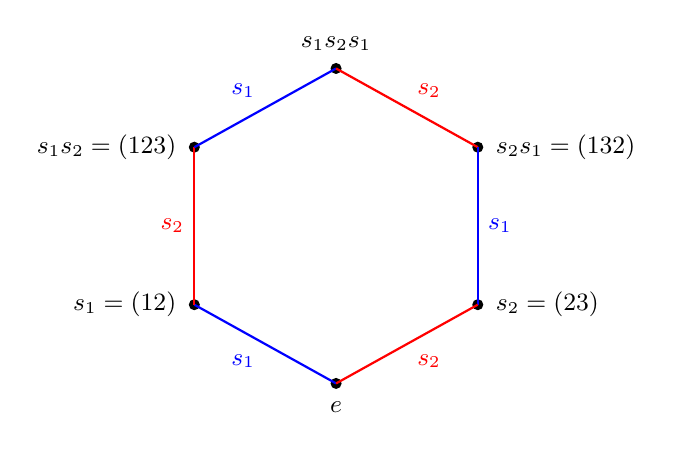
\begin{tikzpicture}[every node/.style={font=\small}]
  \coordinate (e) at (0,-2);
  \coordinate (b) at (1.8,-1);
  \coordinate (ba) at (1.8,1);
  \coordinate (aba) at (0,2);
  \coordinate (ab) at (-1.8,1);
  \coordinate (a) at (-1.8,-1);
  \foreach \p in {e,b,ba,aba,ab,a} { \fill (\p) circle (2pt); }
  \node[below=3pt] at (e) {$e$};
  \node[left=3pt] at (a) {$s_1 = (12)$};
  \node[left=3pt] at (ab) {$s_1 s_2 = (123)$};
  \node[above=3pt] at (aba) {$s_1 s_2 s_1$};
  \node[right=3pt] at (ba) {$s_2 s_1 = (132)$};
  \node[right=3pt] at (b) {$s_2 = (23)$};
  \draw[blue, thick] (e) -- node[below left] {$s_1$} (a);
  \draw[red, thick] (a) -- node[left] {$s_2$} (ab);
  \draw[blue, thick] (ab) -- node[above left] {$s_1$} (aba);
  \draw[red, thick] (aba) -- node[above right] {$s_2$} (ba);
  \draw[blue, thick] (ba) -- node[right] {$s_1$} (b);
  \draw[red, thick] (b) -- node[below right] {$s_2$} (e);
\end{tikzpicture}
